\documentclass[10pt]{beamer}

\usepackage{dcolumn, booktabs}
\newcolumntype{d}[1]{D..{#1}}
\newcommand\mc[1]{\multicolumn{1}{c}{#1}} % handy shortcut macro

\usepackage{tikz}
\usepackage{pgfplots}
\pgfplotsset{compat=1.17}
\usepgfplotslibrary{colorbrewer}
\usepackage{collcell}
\usepackage[latin1]{inputenc}
\usepackage{times}
\usepackage[T1]{fontenc}
\usepackage{pgfpages}
\usepackage{graphicx}

 %The min, mid and max values
\newcommand*{\MinNumber}{-20}%
\newcommand*{\MidNumber}{0} %
\newcommand*{\MaxNumber}{30}%

%Apply the gradient macro
\newcommand{\ApplyGradient}[1]{%
        \ifdim #1 pt > \MidNumber pt
            \pgfmathsetmacro{\PercentColor}{max(min(100.0*(#1 - \MidNumber)/(\MaxNumber-\MidNumber),100.0),0.00)} %
            \hspace{-0.33em}\colorbox{red!\PercentColor!white}{\makebox[2em]{#1}}
            % \colorbox{red!\PercentColor!white}{#1}
        \else
            \pgfmathsetmacro{\PercentColor}{max(min(100.0*(\MidNumber - #1)/(\MidNumber-\MinNumber),100.0),0.00)} %
            \hspace{-0.33em}\colorbox{blue!\PercentColor!white}{\makebox[2em]{#1}}
        \fi
}

\newcolumntype{R}{>{\collectcell\ApplyGradient}r<{\endcollectcell}}
\renewcommand{\arraystretch}{0}
\setlength{\fboxsep}{12pt} % box size
\setlength{\tabcolsep}{0pt}


\mode<presentation> {
  \usetheme{Warsaw}
  \setbeamercovered{transparent}
  
}

\pgfdeclareimage[height=0.7cm]{le-logo}{UZH-logo}
\logo{\pgfuseimage{le-logo}}
\setbeamertemplate{footline}[frame number]
\title{Final Exercise -- Beamer}
\author{Wenying Huang \and Shujun Wang \and Simon Williamn}
\institute{University of Zurich}
\date{\today}


\setbeamertemplate{caption}[numbered]
\setbeamertemplate{theorems}[numbered]

\begin{document}

% ========================


\begin{frame}
  \titlepage
\end{frame}

\begin{frame}{Table of Contents}
  \tableofcontents
\end{frame}

\section{Table}

% ========================

\subsection{Table with DColumn}

\begin{frame}
\frametitle{Table Page}
\framesubtitle{An Example Table with DColumn}

\begin{table}
\centering
\begin{tabular}{@{} l *{3}{d{6.9}} @{}}
  \toprule
  $n$ & \mc{$\nu=1/3$} & \mc{$\nu=1/5$} & \mc{$\nu=1/7$} \\
  \midrule
  1 &         -2.6448(2) &         -3.5613(2) &         -3.7317(2) \\
  2 &          1.0022(1) &          2.8438(1) &          3.4644(1) \\
  3 &          0.0613(4) &         -1.8256(4) &         -3.0903(4) \\
  4 &         -0.4103(4) &          0.7144(4) &          2.4534(4) \\
  \bottomrule
\end{tabular}
\caption{Expansion coefficients for various filling factors.}
\end{table}

\end{frame}

% ========================

\subsection{Table with Heatmap}
\begin{frame}
\frametitle{Another Table Page}
\framesubtitle{An Example Table with Heatmap}

\begin{table}
\footnotesize
\centering
\begin{tabular}{ *{5}{R} }
2.9 & 4.6 & 9.5 & 13.8 & 18.5 \\
0.3 & 1.3 & 5.3 & 8.8 & 13.3 \\
-2.0 & -1.6 & 1.7 & 4.5 & 8.8 \\
\end{tabular}
\caption{Heatmap Table}
\end{table}

\end{frame}
% ========================

\section{Figure}
\subsection{Figure with Color Palette}
\begin{frame}
\frametitle{Figure Page}
\framesubtitle{An Example Figure with Color Palette}
\begin{figure}
\centering

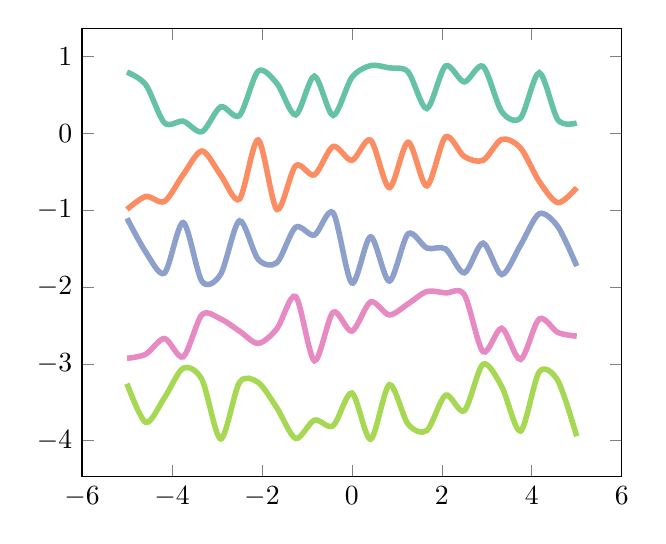
\begin{tikzpicture}
\begin{axis}[smooth, cycle list/Set2]
    \addplot +[line width=2pt] {rnd};
    \addplot +[line width=2pt] {rnd-1};
    \addplot +[line width=2pt] {rnd-2};
    \addplot +[line width=2pt] {rnd-3};
    \addplot +[line width=2pt] {rnd-4};
\end{axis}
\end{tikzpicture}
\caption{Figure with color palette}

\end{figure}
\end{frame}

% ========================

\subsection{Figure with Two Panels}
\begin{frame}
\frametitle{Another Figure Page}
\framesubtitle{An Example Figure with two panels}
\begin{figure}
\centering
\begin{minipage}[b]{0.45\textwidth}

\includegraphics[width=\linewidth]{UZH-logo.png}
\caption{UZH logo}
\end{minipage}
\begin{minipage}[b]{0.45\textwidth}

\includegraphics[width=\linewidth]{ETH-logo.png}
\caption{ETH logo}
\end{minipage}
\end{figure}
\end{frame}

% ========================

\section{Equation}
\begin{frame}
\frametitle{Equation Page}
\framesubtitle{Equations}
Mass-Energy Equivalence:
\begin{equation}
E=mc^2
\end{equation}
Euler's Identity:
\begin{equation}
e^{i\pi}+1=0
\end{equation}
\end{frame}

% ========================

\section{Theorem}
\begin{frame}
\frametitle{Theorem Page}
\framesubtitle{Theorem and proof}
\begin{theorem}
Dummy theorem.
\end{theorem}
\begin{proof}
Dummy proof.
\end{proof}
\end{frame}

% ========================


\end{document}
